\batchmode
\makeatletter
\def\input@path{{/home/erik/work/svnwc/rcolgem/pkg/rcolgem/vignettes//}}
\makeatother
\documentclass[english]{article}\usepackage[]{graphicx}\usepackage[]{color}
%% maxwidth is the original width if it is less than linewidth
%% otherwise use linewidth (to make sure the graphics do not exceed the margin)
\makeatletter
\def\maxwidth{ %
  \ifdim\Gin@nat@width>\linewidth
    \linewidth
  \else
    \Gin@nat@width
  \fi
}
\makeatother

\definecolor{fgcolor}{rgb}{0.345, 0.345, 0.345}
\newcommand{\hlnum}[1]{\textcolor[rgb]{0.686,0.059,0.569}{#1}}%
\newcommand{\hlstr}[1]{\textcolor[rgb]{0.192,0.494,0.8}{#1}}%
\newcommand{\hlcom}[1]{\textcolor[rgb]{0.678,0.584,0.686}{\textit{#1}}}%
\newcommand{\hlopt}[1]{\textcolor[rgb]{0,0,0}{#1}}%
\newcommand{\hlstd}[1]{\textcolor[rgb]{0.345,0.345,0.345}{#1}}%
\newcommand{\hlkwa}[1]{\textcolor[rgb]{0.161,0.373,0.58}{\textbf{#1}}}%
\newcommand{\hlkwb}[1]{\textcolor[rgb]{0.69,0.353,0.396}{#1}}%
\newcommand{\hlkwc}[1]{\textcolor[rgb]{0.333,0.667,0.333}{#1}}%
\newcommand{\hlkwd}[1]{\textcolor[rgb]{0.737,0.353,0.396}{\textbf{#1}}}%

\usepackage{framed}
\makeatletter
\newenvironment{kframe}{%
 \def\at@end@of@kframe{}%
 \ifinner\ifhmode%
  \def\at@end@of@kframe{\end{minipage}}%
  \begin{minipage}{\columnwidth}%
 \fi\fi%
 \def\FrameCommand##1{\hskip\@totalleftmargin \hskip-\fboxsep
 \colorbox{shadecolor}{##1}\hskip-\fboxsep
     % There is no \\@totalrightmargin, so:
     \hskip-\linewidth \hskip-\@totalleftmargin \hskip\columnwidth}%
 \MakeFramed {\advance\hsize-\width
   \@totalleftmargin\z@ \linewidth\hsize
   \@setminipage}}%
 {\par\unskip\endMakeFramed%
 \at@end@of@kframe}
\makeatother

\definecolor{shadecolor}{rgb}{.97, .97, .97}
\definecolor{messagecolor}{rgb}{0, 0, 0}
\definecolor{warningcolor}{rgb}{1, 0, 1}
\definecolor{errorcolor}{rgb}{1, 0, 0}
\newenvironment{knitrout}{}{} % an empty environment to be redefined in TeX

\usepackage{alltt}
\usepackage[T1]{fontenc}
\usepackage[latin9]{inputenc}
\usepackage{url}
\usepackage{amsmath}
\usepackage{amssymb}
\usepackage{babel}
\IfFileExists{upquote.sty}{\usepackage{upquote}}{}
\begin{document}

\title{Fitting a simple HIV model (rcolgem)}


\author{Erik M Volz}

\maketitle
This vignette will demonstrate fitting a simple deterministic HIV
model to a virus genealogy reconstructed from a random sample of 200
patients. The virus genealogy also includes information about the
state of patients at the time of sampling. Note that in a real world
application, it is not always wise to fit a deterministic model to
noisy epidemic data collected from a small population. But, as we
will see, the coalescent based on a deterministic model actually performs
very well in this particular scenario. Furthermore, the coalescent
is robust to sampling a large fraction of infections (61\% in this
scenario). 

People infected with HIV have a period of intensified transmission
shortly after infection, which is due, in part, to higher viral loads
during this period. We will model this using a 2 stage model. $I_{0}$and
$I_{1}$will denote the number of infected in the first and second
stages. The first stage will last $1/\gamma_{0}=1$ year on average,
and the second stage will last $1/\gamma_{1}=9$ years on average,
and we will presume that parameters describing the duration of these
stages are known. The epidemiological dynamics are described by the
following rate equations: 

\begin{align}
S & \xrightarrow{\beta_0 I_0 S + \beta_1 I_1 S} I_0 \\
I_0 &\xrightarrow{ \gamma_0 I_0 } I_1 \\
I_1 &\xrightarrow{ \gamma_1 I_1 } 0 
\end{align}

The objective of this excercise will be to estimate the transmission
rates $\beta_{0}$ and $\beta_{1}$as well as the prevalence of infection
over time. New susceptibles will be born into the population at the
rate $Sb=S/100$ per year, and we will assume this parameter is known. 

Before we begin, we must satisfy a few dependencies. To use rcolgem: 

\begin{knitrout}
\definecolor{shadecolor}{rgb}{0.969, 0.969, 0.969}\color{fgcolor}\begin{kframe}
\begin{alltt}
\hlkwd{require}\hlstd{(rcolgem)}
\end{alltt}


{\ttfamily\noindent\itshape\color{messagecolor}{\#\# Loading required package: rcolgem}}\end{kframe}
\end{knitrout}


We will also need the following packages:

\begin{knitrout}
\definecolor{shadecolor}{rgb}{0.969, 0.969, 0.969}\color{fgcolor}\begin{kframe}
\begin{alltt}
\hlkwd{require}\hlstd{(deSolve)}  \hlcom{# solves ODEs}
\end{alltt}


{\ttfamily\noindent\itshape\color{messagecolor}{\#\# Loading required package: deSolve}}\begin{alltt}
\hlkwd{require}\hlstd{(ape)}  \hlcom{# for working with phylogenies}
\end{alltt}


{\ttfamily\noindent\itshape\color{messagecolor}{\#\# Loading required package: ape}}\begin{alltt}
\hlkwd{require}\hlstd{(rjson)}  \hlcom{# for loading simulation data}
\end{alltt}


{\ttfamily\noindent\itshape\color{messagecolor}{\#\# Loading required package: rjson}}\begin{alltt}
\hlkwd{require}\hlstd{(stats4)}  \hlcom{# for fitting models by maximum likelihood}
\end{alltt}


{\ttfamily\noindent\itshape\color{messagecolor}{\#\# Loading required package: stats4\\\#\# Loading required package: methods}}\end{kframe}
\end{knitrout}


We will use simulated data for this vignette. Data were simulated
using MASTER 1.4.1 (\url{http://tgvaughan.github.io/MASTER/}). You
can find the xml file used to configure the simulation in ``extdata``
folder of your package installation directory. To load the simulated
data: 

\begin{knitrout}
\definecolor{shadecolor}{rgb}{0.969, 0.969, 0.969}\color{fgcolor}\begin{kframe}
\begin{alltt}
\hlstd{hivSimulationData} \hlkwb{<-} \hlkwd{fromJSON}\hlstd{(}
  \hlkwc{file}\hlstd{=} \hlkwd{system.file}\hlstd{(}\hlstr{'extdata/HIVModel.json'}\hlstd{,} \hlkwc{package} \hlstd{=} \hlstr{"rcolgem"}\hlstd{) )}
\hlstd{tree} \hlkwb{<-} \hlkwd{read.tree}\hlstd{(} \hlkwd{system.file}\hlstd{(}\hlstr{'extdata/HIVModel.nwk'}\hlstd{,} \hlkwc{package} \hlstd{=} \hlstr{"rcolgem"}\hlstd{) )}
\end{alltt}
\end{kframe}
\end{knitrout}


Before fitting the model to the tree, let's visualize the data: 

\begin{knitrout}
\definecolor{shadecolor}{rgb}{0.969, 0.969, 0.969}\color{fgcolor}\begin{kframe}
\begin{alltt}
\hlkwd{with}\hlstd{(hivSimulationData,}
\hlstd{\{} \hlkwd{plot}\hlstd{(t, S,} \hlstr{'l'}\hlstd{,} \hlkwc{ylim}\hlstd{=}\hlkwd{c}\hlstd{(}\hlnum{0}\hlstd{,} \hlkwd{max}\hlstd{(S)),} \hlkwc{col}\hlstd{=}\hlstr{'blue'}\hlstd{,}
  \hlkwc{main}\hlstd{=}\hlstr{'Number infected, red=stage0, orange=stage1'}\hlstd{,}
  \hlkwc{xlab}\hlstd{=}\hlstr{'time'}\hlstd{,} \hlkwc{ylab}\hlstd{=}\hlstr{''}\hlstd{)}
\hlkwd{lines}\hlstd{(t, I0,} \hlkwc{col}\hlstd{=}\hlstr{'red'}\hlstd{)}
\hlkwd{lines}\hlstd{(t, I1,} \hlkwc{col}\hlstd{=}\hlstr{'orange'}\hlstd{) \})}
\end{alltt}
\end{kframe}
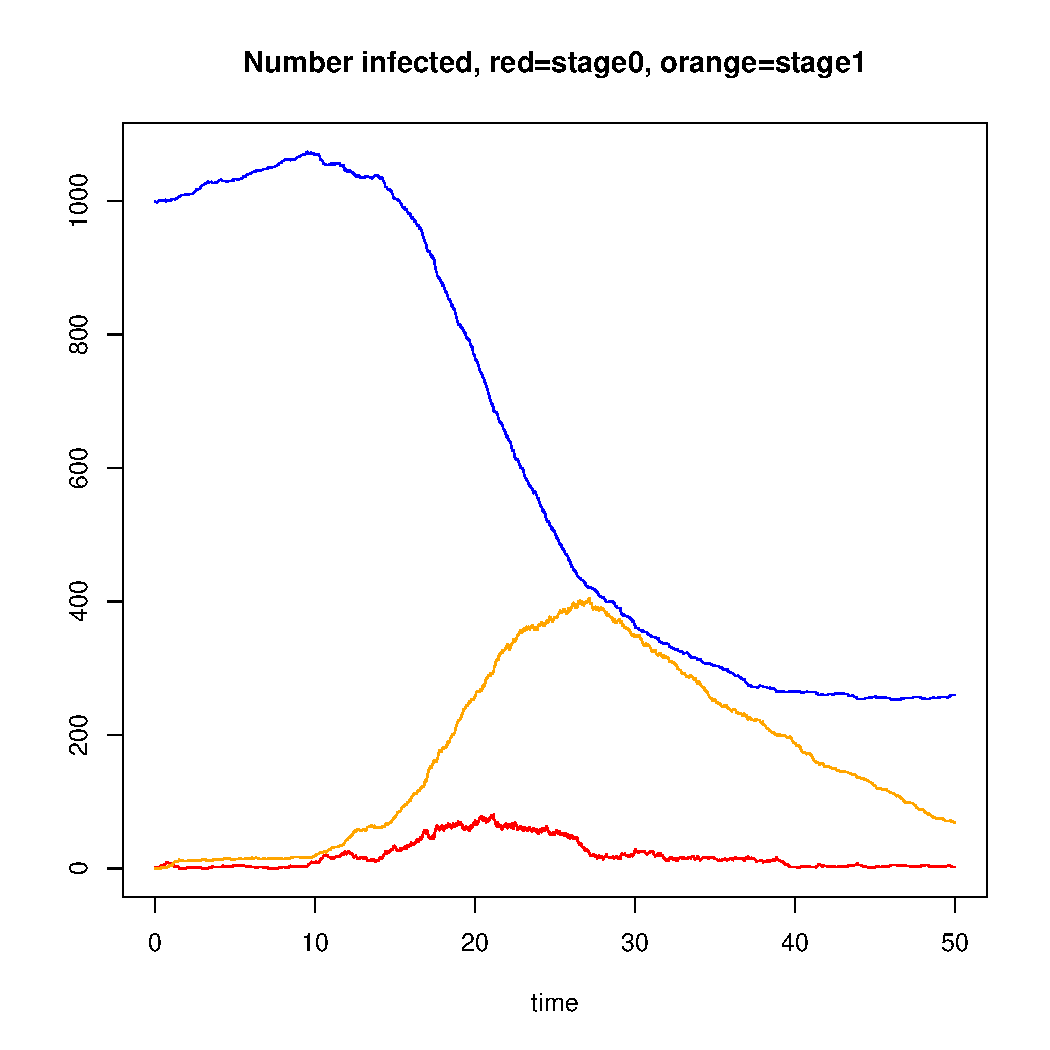
\includegraphics[width=\maxwidth]{figure/unnamed-chunk-4} 

\end{knitrout}


And, we can visualize the tree using the ape package: 

\begin{knitrout}
\definecolor{shadecolor}{rgb}{0.969, 0.969, 0.969}\color{fgcolor}\begin{kframe}
\begin{alltt}
\hlkwd{plot.phylo}\hlstd{(tree,} \hlkwc{show.tip.label} \hlstd{=} \hlnum{FALSE}\hlstd{)}
\end{alltt}
\end{kframe}
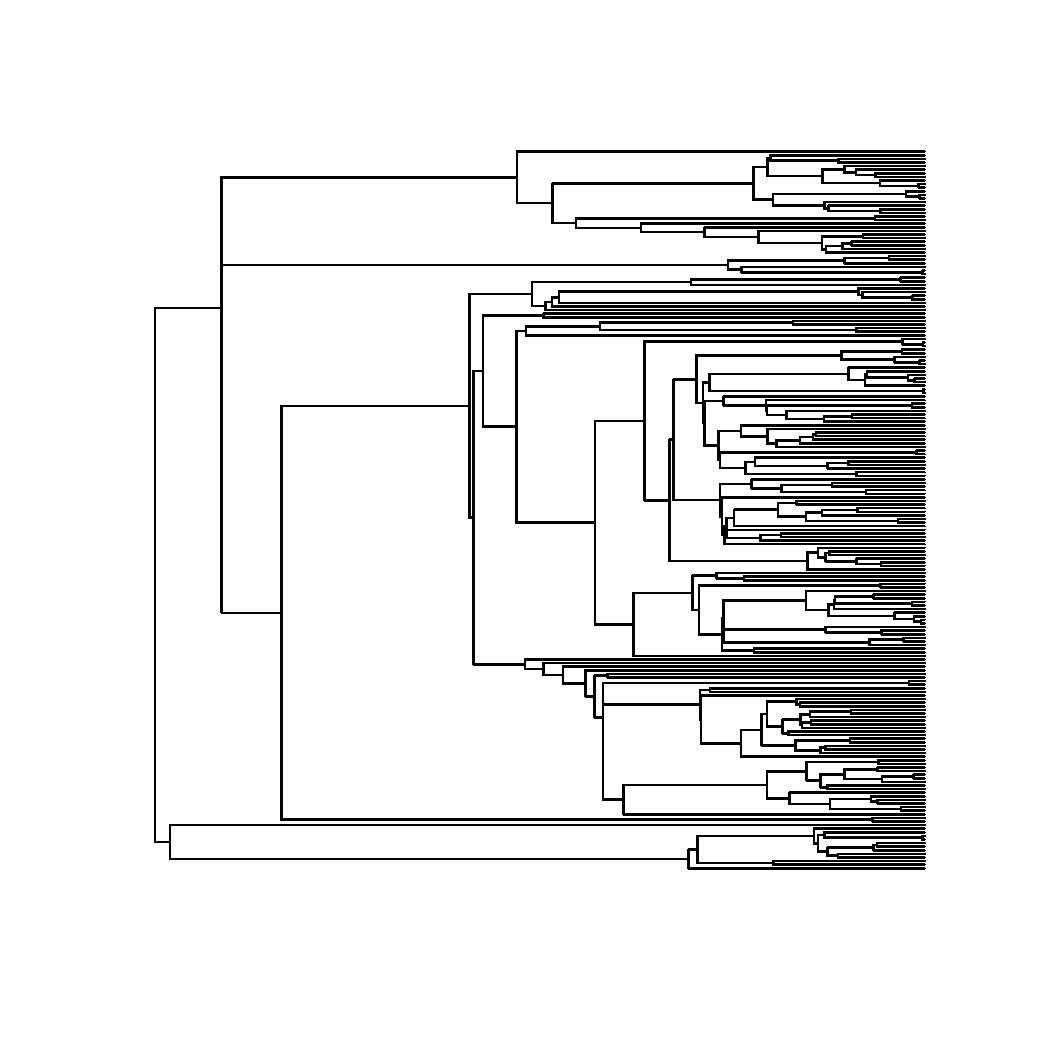
\includegraphics[width=\maxwidth]{figure/unnamed-chunk-5} 

\end{knitrout}


These are the true parameter values:

\begin{knitrout}
\definecolor{shadecolor}{rgb}{0.969, 0.969, 0.969}\color{fgcolor}\begin{kframe}
\begin{alltt}
\hlstd{S0} \hlkwb{<-} \hlnum{999}\hlstd{;} \hlcom{# the initial number susceptible}
\hlstd{sampleTime} \hlkwb{<-} \hlnum{20}\hlstd{;} \hlcom{# the last time point in the simulation }
\hlstd{beta0} \hlkwb{<-} \hlnum{.001}\hlstd{;} \hlcom{#the true transmission rate per person per year for stage 0 infected}
\hlstd{beta1} \hlkwb{<-} \hlnum{.0001}\hlstd{;} \hlcom{#the true transmission rate per person per year for stage 1 infected}
\hlstd{gamma0} \hlkwb{<-} \hlnum{1}\hlstd{;} \hlcom{# the rate that infected progress from stage 0 to stage 1 per person per year }
\hlstd{gamma1} \hlkwb{<-} \hlnum{0.1111}\hlstd{;} \hlcom{# the rate that stage 1 infected progress to death per person per year }
\hlstd{b} \hlkwb{<-} \hlnum{.01} \hlcom{# the per capita birth rate of new susceptibles}
\end{alltt}
\end{kframe}
\end{knitrout}


Note that the tree contains information about the state of patients
at the time of sampling in the tree\$tip.label attribute. Patients
sampled in stage 0 have a label that ends in 'Y0', and patients sampled
in state 1 have a label that ends in 'Y1'. We will use this information
when fitting the model, so we need to extract it from the tree. The
following code generates a vector of sample states corresponding to
each tip in the tree:

\begin{knitrout}
\definecolor{shadecolor}{rgb}{0.969, 0.969, 0.969}\color{fgcolor}\begin{kframe}
\begin{alltt}
\hlstd{calcStateFromName} \hlkwb{<-} \hlkwa{function}\hlstd{(}\hlkwc{tl}\hlstd{) \{}
    \hlstd{lentl} \hlkwb{<-} \hlkwd{nchar}\hlstd{(tl)}
    \hlstd{tailstr} \hlkwb{<-} \hlkwd{substr}\hlstd{(tl, lentl} \hlopt{-} \hlnum{1}\hlstd{, lentl)}
    \hlkwa{if} \hlstd{(tailstr} \hlopt{==} \hlstr{"I0"}\hlstd{) \{}
        \hlkwd{return}\hlstd{(}\hlkwd{c}\hlstd{(}\hlnum{1}\hlstd{,} \hlnum{0}\hlstd{))}
    \hlstd{\}}
    \hlkwd{return}\hlstd{(}\hlkwd{c}\hlstd{(}\hlnum{0}\hlstd{,} \hlnum{1}\hlstd{))}
\hlstd{\}}
\hlstd{sampleStates} \hlkwb{<-} \hlkwd{t}\hlstd{(}\hlkwd{sapply}\hlstd{(tree}\hlopt{$}\hlstd{tip.label, calcStateFromName))}
\end{alltt}
\end{kframe}
\end{knitrout}


We will also need to know the time of sampling of each patient. In
this case, we are working with a 'homochronous' sample-- everyone
was sampled at the same point in time at the end of the simulation: 

\begin{knitrout}
\definecolor{shadecolor}{rgb}{0.969, 0.969, 0.969}\color{fgcolor}\begin{kframe}
\begin{alltt}
\hlstd{sampleTimes} \hlkwb{<-} \hlkwd{rep}\hlstd{(sampleTime,} \hlkwd{length}\hlstd{(tree}\hlopt{$}\hlstd{tip.label))}
\end{alltt}
\end{kframe}
\end{knitrout}


Now we are ready to create a 'binaryDatedTree' object which extends
the ape::phylo class. The binaryDatedTree includes the sample time
and state information and also calculates the 'height' of each node-
that is, the time in the past of each node in the tree relative to
the most recent sample. 

\begin{knitrout}
\definecolor{shadecolor}{rgb}{0.969, 0.969, 0.969}\color{fgcolor}\begin{kframe}
\begin{alltt}
\hlstd{bdt} \hlkwb{<-} \hlkwd{binaryDatedTree}\hlstd{(tree, sampleTimes, sampleStates)}
\end{alltt}
\end{kframe}
\end{knitrout}


Finally, we are ready to define the model to be fitted. The model
is described by the following ODEs:

\begin{align}
\dot{S} &= b S - \beta_0 I_0 - \beta_1 I_1 \\
\dot{I_0} &= \beta_0 I_0 + \beta_1 I_1 - \gamma_0 I_0  \\
\dot{I_1} &= \gamma_0 I_0 - \gamma_1 I_1
\end{align}

We need to transform this model into a canonical form so that it can
be used for coalescent calculations. To do that, we must decompose
this model into a set of births (replication of lineages within and
between states) and migrations (changes of state). A lineage in this
model can occupy two states ($I_{0}$or $I_{1}$) even though there
are three equations, so we must tabulate births and migrations between
two states. Note that an equivalent way to write the model is

\begin{align}
\dot{I_0}(t) &= F_{00}(t) + F_{10}(t) - G_{01}(t) - \mathrm{deaths}_0(t) \\
\dot{I_1}(t) &= F_{11}(t) + F_{01}(t) - G_{10}(t) - \mathrm{deaths}_1(t) \\
\end{align}

where $F(t)$ is a 2x2 matrix of birth rates and $G(t)$is a 2x2 matrix
of migration rates. This decomposition is valid for any epidemiological
model with two states. In our HIV model, we have

\begin{align}
F_{00}(t) &= \beta_0 I_0 S \\
F_{01}(t) &= \beta_1 I_1 S \\
G_{01}(t) &= \gamma_0 I_0 \\
\mathrm{deaths}_1 &= \gamma_1 I_1,
\end{align}

with all other elements zero. 

The following R code is a re-statement of the above discussion:

\begin{knitrout}
\definecolor{shadecolor}{rgb}{0.969, 0.969, 0.969}\color{fgcolor}\begin{kframe}
\begin{alltt}
\hlstd{FofX} \hlkwb{<-} \hlkwa{function}\hlstd{(}\hlkwc{X}\hlstd{,} \hlkwc{param}\hlstd{) \{}
        \hlkwd{return}\hlstd{(}  \hlkwd{matrix}\hlstd{(} \hlkwd{rbind}\hlstd{(}
                \hlkwd{c}\hlstd{(X[}\hlstr{'I0'}\hlstd{]} \hlopt{*} \hlstd{X[}\hlstr{'S'}\hlstd{]} \hlopt{*} \hlstd{param}\hlopt{$}\hlstd{beta0,} \hlnum{0}\hlstd{),}
                \hlkwd{c}\hlstd{(X[}\hlstr{'I1'}\hlstd{]} \hlopt{*} \hlstd{X[}\hlstr{'S'}\hlstd{]} \hlopt{*} \hlstd{param}\hlopt{$}\hlstd{beta1,} \hlnum{0}\hlstd{))}
\hlstd{,} \hlnum{2}\hlstd{,}\hlnum{2}\hlstd{))  \}}

\hlstd{GofX} \hlkwb{<-} \hlkwa{function}\hlstd{(}\hlkwc{X}\hlstd{,} \hlkwc{param}\hlstd{)\{}
        \hlkwd{return}\hlstd{(} \hlkwd{matrix}\hlstd{(} \hlkwd{rbind}\hlstd{(}
                \hlkwd{c}\hlstd{(}\hlnum{0}\hlstd{, X[}\hlstr{'I0'}\hlstd{]} \hlopt{*} \hlstd{param}\hlopt{$}\hlstd{gamma0 ),}
                \hlkwd{c}\hlstd{(}\hlnum{0}\hlstd{,} \hlnum{0}\hlstd{))}
\hlstd{,} \hlnum{2}\hlstd{,}\hlnum{2} \hlstd{) ) \}}
\end{alltt}
\end{kframe}
\end{knitrout}


This defines the ODEs in R:

\begin{knitrout}
\definecolor{shadecolor}{rgb}{0.969, 0.969, 0.969}\color{fgcolor}\begin{kframe}
\begin{alltt}
\hlstd{dX} \hlkwb{<-} \hlkwa{function}\hlstd{(}\hlkwc{t}\hlstd{,} \hlkwc{X}\hlstd{,} \hlkwc{param}\hlstd{,} \hlkwc{...}\hlstd{) \{}
  \hlcom{# X == S, I0, I1}
  \hlstd{.F} \hlkwb{<-} \hlkwd{FofX}\hlstd{(X, param)}
  \hlstd{.G} \hlkwb{<-} \hlkwd{GofX}\hlstd{(X, param)}
  \hlkwd{list}\hlstd{(}\hlkwd{unname}\hlstd{(}\hlkwd{c}\hlstd{(}
    \hlopt{-}\hlkwd{sum}\hlstd{(.F)} \hlopt{+} \hlstd{param}\hlopt{$}\hlstd{b} \hlopt{*} \hlstd{X[}\hlstr{'S'}\hlstd{],}
    \hlkwd{sum}\hlstd{(.F)} \hlopt{-} \hlkwd{sum}\hlstd{(.G),}
    \hlkwd{sum}\hlstd{(.G)} \hlopt{-} \hlstd{param}\hlopt{$}\hlstd{gamma1} \hlopt{*} \hlstd{X[}\hlstr{'I1'}\hlstd{]  ))) \}}
\end{alltt}
\end{kframe}
\end{knitrout}


Now we need to define a function to integrate the model equations
and calculate the likelihood. The rcolgem package provides the 'coalescent.log.likelihood'
function which calculate the log likelihood of a given binaryDatedTree.
This function expects several global variables to be defined, namely
'F.', 'G.', and 'Y.'. These are functions of time which respectively
represent the matrix of births, migrations, and population size through
time, and one must integrate the system of ODEs for a given set of
parameters before defining these global variables. 

\begin{knitrout}
\definecolor{shadecolor}{rgb}{0.969, 0.969, 0.969}\color{fgcolor}\begin{kframe}
\begin{alltt}
\hlstd{integrate.model.calculate.minusLogLikelihood} \hlkwb{<-} \hlkwa{function}\hlstd{(}\hlkwc{logbeta0}\hlstd{,} \hlkwc{logbeta1}\hlstd{) \{}
    \hlstd{param} \hlkwb{<-} \hlkwd{list}\hlstd{(}\hlkwc{beta0} \hlstd{=} \hlkwd{unname}\hlstd{(}\hlkwd{exp}\hlstd{(logbeta0)),} \hlkwc{beta1} \hlstd{=} \hlkwd{unname}\hlstd{(}\hlkwd{exp}\hlstd{(logbeta1)),}
        \hlkwc{gamma0} \hlstd{= gamma0,} \hlkwc{gamma1} \hlstd{= gamma1,} \hlkwc{b} \hlstd{= b)}
    \hlstd{X0} \hlkwb{<-} \hlkwd{c}\hlstd{(}\hlkwc{S} \hlstd{= S0,} \hlkwc{I0} \hlstd{=} \hlnum{1}\hlstd{,} \hlkwc{I1} \hlstd{=} \hlnum{0}\hlstd{)}
    \hlstd{times} \hlkwb{<-} \hlkwd{seq}\hlstd{(}\hlnum{0}\hlstd{,} \hlnum{35}\hlstd{,} \hlkwc{length.out} \hlstd{=} \hlnum{100}\hlstd{)}
    \hlkwd{tryCatch}\hlstd{(\{}
        \hlstd{o} \hlkwb{<-} \hlkwd{ode}\hlstd{(X0, times, dX, param)}
    \hlstd{\},} \hlkwc{error} \hlstd{=} \hlkwa{function}\hlstd{(}\hlkwc{e}\hlstd{) \{}
        \hlkwd{return}\hlstd{(}\hlnum{Inf}\hlstd{)}
    \hlstd{\})}
    \hlstd{S} \hlkwb{<-} \hlkwd{approxfun}\hlstd{(o[,} \hlnum{1}\hlstd{], o[,} \hlnum{2}\hlstd{])}
    \hlstd{Y1} \hlkwb{<-} \hlkwd{approxfun}\hlstd{(o[,} \hlnum{1}\hlstd{], o[,} \hlnum{3}\hlstd{])}
    \hlstd{Y2} \hlkwb{<-} \hlkwd{approxfun}\hlstd{(o[,} \hlnum{1}\hlstd{], o[,} \hlnum{4}\hlstd{])}
    \hlstd{Y.} \hlkwb{<<-} \hlkwa{function}\hlstd{(}\hlkwc{t}\hlstd{) \{}
        \hlkwd{c}\hlstd{(}\hlkwc{I0} \hlstd{=} \hlkwd{Y1}\hlstd{(t),} \hlkwc{I1} \hlstd{=} \hlkwd{Y2}\hlstd{(t))}
    \hlstd{\}}
    \hlstd{F.} \hlkwb{<<-} \hlkwa{function}\hlstd{(}\hlkwc{t}\hlstd{) \{}
        \hlkwd{FofX}\hlstd{(}\hlkwd{c}\hlstd{(}\hlkwc{S} \hlstd{=} \hlkwd{S}\hlstd{(t),} \hlkwd{Y.}\hlstd{(t)), param)}
    \hlstd{\}}
    \hlstd{G.} \hlkwb{<<-} \hlkwa{function}\hlstd{(}\hlkwc{t}\hlstd{) \{}
        \hlkwd{GofX}\hlstd{(}\hlkwd{c}\hlstd{(}\hlkwc{S} \hlstd{=} \hlkwd{S}\hlstd{(t),} \hlkwd{Y.}\hlstd{(t)), param)}
    \hlstd{\}}
    \hlkwd{return}\hlstd{(}\hlopt{-}\hlkwd{coalescent.log.likelihood}\hlstd{(bdt))}
\hlstd{\}}
\end{alltt}
\end{kframe}
\end{knitrout}


Note that this function takes two arguments which are the parameters
to be estimated. These are log-transformed because the domain of these
variables is $(0,\infty)$. 

The coalescent.log.likelihood function takes two optional arguments:
integrationMethod describes the integration method used by the deSolve
package. The default 'rk4' option is fast, but not very accurate.
You may find that switching to 'adams' improves performance. 

The finiteSizeCorrections option (default=FALSE), tells the coalescent.log.likelihood
function whether to carry out additional adjustments for small population
sizes. Setting this option to TRUE will be important for certain applications
with very small population sizes (such as near the beginning of an
epidemic) and where the number of lineages in the tree is close to
the population size. For the HIV example, we find acceptable results
with the option set to FALSE. 

Now we can fit the model using the stats4 package. NOTE: this will
take a few minutes! 

\begin{knitrout}
\definecolor{shadecolor}{rgb}{0.969, 0.969, 0.969}\color{fgcolor}\begin{kframe}
\begin{alltt}
\hlstd{fit} \hlkwb{<-} \hlkwd{mle}\hlstd{(integrate.model.calculate.minusLogLikelihood,}
           \hlkwc{start} \hlstd{=} \hlkwd{list}\hlstd{(} \hlkwc{logbeta0}\hlstd{=}\hlkwd{log}\hlstd{(beta0}\hlopt{/}\hlnum{2}\hlstd{),}\hlkwc{logbeta1}\hlstd{=}\hlkwd{log}\hlstd{(beta1}\hlopt{*}\hlnum{2}\hlstd{)),}
           \hlkwc{method}\hlstd{=}\hlstr{'Nelder-Mead'}\hlstd{,}
           \hlkwc{control}\hlstd{=}\hlkwd{list}\hlstd{(}\hlkwc{maxit}\hlstd{=}\hlnum{1000} \hlstd{) )}
\end{alltt}
\end{kframe}
\end{knitrout}


Let's inspect the output: 

\begin{knitrout}
\definecolor{shadecolor}{rgb}{0.969, 0.969, 0.969}\color{fgcolor}\begin{kframe}
\begin{alltt}
\hlkwd{summary}\hlstd{(fit)}
\end{alltt}
\begin{verbatim}
## Maximum likelihood estimation
## 
## Call:
## mle(minuslogl = integrate.model.calculate.minusLogLikelihood, 
##     start = list(logbeta0 = log(beta0/2), logbeta1 = log(beta1 * 
##         2)), method = "Nelder-Mead", control = list(maxit = 1000))
## 
## Coefficients:
##          Estimate Std. Error
## logbeta0   -6.774    0.01273
## logbeta1   -9.403    0.06109
## 
## -2 log L: 2359
\end{verbatim}
\begin{alltt}
\hlkwd{unname}\hlstd{(}\hlkwd{exp}\hlstd{(}\hlkwd{coef}\hlstd{(fit)))}  \hlcom{# the untransformed parameter estimates}
\end{alltt}
\begin{verbatim}
## [1] 1.143e-03 8.251e-05
\end{verbatim}
\begin{alltt}
\hlkwd{AIC}\hlstd{(fit)}
\end{alltt}
\begin{verbatim}
## [1] 2363
\end{verbatim}
\begin{alltt}
\hlcom{# bias relative to true values:}
\hlkwd{unname}\hlstd{(}\hlkwd{c}\hlstd{(beta0, beta1)} \hlopt{-} \hlkwd{exp}\hlstd{(}\hlkwd{coef}\hlstd{(fit)))}
\end{alltt}
\begin{verbatim}
## [1] -1.432e-04  1.749e-05
\end{verbatim}
\end{kframe}
\end{knitrout}


%We can also calculate approximate confidence intervals using the approximate standard errors from the 'mle' object. More accurate confidence intervals could be found using the profile(fit) function, but that would take a long time. I recommend using the more robust version of profile in the bbmle package. %<<>>=
%cis <- unname( rbind( 
%	exp(coef(fit) - diag( sqrt( vcov(fit) )) * 1.96 ),   
%	exp( coef(fit) + diag( sqrt( vcov(fit) )) * 1.96 ) ) )  
%colnames(cis) <- c('beta0', 'beta1') 
%cis
%@
\end{document}
